% Graph G and all possible spanning trees
\begin{figure}[htb]
\centering
\subfigure
{
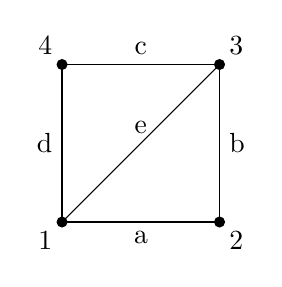
\begin{tikzpicture}[scale=2,baseline=(current bounding box.center)]

\node (n1) at (0,0) {};
\node (n2) at (1,0) {};
\node (n3) at (1,1) {};
\node (n4) at (0,1) {};

\draw (n1) node[anchor=north east] {$1$};
\draw (n2) node[anchor=north west] {$2$};
\draw (n3) node[anchor=south west] {$3$};
\draw (n4) node[anchor=south east] {$4$};

\foreach \i in {1,...,4}
{
	\fill (n\i) circle [radius=1pt];
};

\foreach \i/ \j/ \label/\position in {1/2/a/below, 2/3/b/right, 
					3/4/c/above, 4/1/d/left, 
					1/3/e/above}
{
	\path (n\i.center) edge node[\position] {\label} (n\j.center);
};
\end{tikzpicture}
}
\subfigure
{
  \def\graph#1{%
    \begin{tikzpicture}
    \node (n1) at (0,0) {};
    \node (n2) at (1,0) {};
    \node (n3) at (1,1) {};
    \node (n4) at (0,1) {};
    \foreach \i in {1,...,4}
       \fill (n\i) circle [radius=2pt];
    \foreach \i / \j in {#1}
        \path (n\i.center) edge (n\j.center);
    \end{tikzpicture}%
  }
  \begin{tabular}{cccc}
    \graph{2/3, 3/4, 4/1} &
    \graph{1/2, 3/4, 4/1} &
    \graph{1/2, 2/3, 4/1} &
    \graph{1/2, 2/3, 3/4} \\
    \graph{1/2, 3/4, 1/3} &
    \graph{2/3, 4/1, 1/3} &
    \graph{2/3, 3/4, 1/3} &
    \graph{1/2, 4/1, 1/3} \\
  \end{tabular}
}
\caption{Graph $G$ and all its spanning trees}
\end{figure}



